\documentclass[preview]{standalone}
\usepackage{graphicx}
% xyqcirc stuff
\usepackage[frame,line,arrow,matrix,tips]{xy}	% all that is usually necessary
\begin{document}

% begin qasm2circ
%
% File:	  algorithm.qasm
% Date:	  17-Nov-21
% Author: G. Huebner
%
% 
%     def ry,0,'\txt{R\textsubscript{y}}'
%     def cry,1,'\txt{R\textsubscript{y}}'
%     def cry2,2,'\txt{R\textsubscript{y}}'
% 
%     defbox chall,4,1,'\txt{H\textsubscript{ALL}}'
%     defbox chall1,4,2,'\txt{H\textsubscript{ALL}}'
%     def chall2,3,'\txt{H\textsubscript{ALL}}'
% 
%     qubit q0,0
%     qubit q1,0
%     qubit q2,0
%     qubit q3,0
% 
%     ry q0
%     chall q0,q1,q2,q3
%     X q0
% 
%     cry q0,q1
%     chall1 q0,q1,q2,q3
%     X q1
% 
%     cry2 q0,q1,q2
%     chall2 q0,q1,q2,q3
%     X q2
% 
%     nop q0
%     nop q1
%     nop q3
% 
%     measure q0
%     measure q1
%     measure q2
%     measure q3
%  Time 01:
%    Gate 00 ry(q0)
%  Time 02:
%    Gate 01 chall(q0,q1,q2,q3)
%  Time 03:
%    Gate 02 X(q0)
%  Time 04:
%    Gate 03 cry(q0,q1)
%  Time 05:
%    Gate 04 chall1(q0,q1,q2,q3)
%  Time 06:
%    Gate 05 X(q1)
%  Time 07:
%    Gate 06 cry2(q0,q1,q2)
%  Time 08:
%    Gate 07 chall2(q0,q1,q2,q3)
%  Time 09:
%    Gate 08 X(q2)
%    Gate 09 nop(q0)
%    Gate 10 nop(q1)
%    Gate 11 nop(q3)
%  Time 10:
%    Gate 12 measure(q0)
%    Gate 13 measure(q1)
%    Gate 14 measure(q2)
%    Gate 15 measure(q3)

% Qubit circuit matrix:
%
% q0: gAxA, gBxA, gCxA, gDxA, gExA, n  , gGxA, gHxA, gIxA, gJxA, N  
% q1: n  , gBxB, n  , gDxB, gExB, gFxB, gGxB, gHxB, gIxB, gJxB, N  
% q2: n  , gBxC, n  , n  , gExC, n  , gGxC, gHxC, gIxC, gJxC, N  
% q3: n  , gBxD, n  , n  , gExD, n  , n  , gHxD, gIxD, gJxD, N  

%
% File:   xyqcirc.tex
% Date:   14-Mar-04
% Author: I. Chuang <ichuang@mit.edu>
%
% Definitions for producing quantum circuits with XYPIC in latex
%
% $Log: xyqcirc.tex,v $
% Revision 1.17  2004/03/25 05:01:23  ike
% discard and slash
%
% Revision 1.16  2004/03/25 04:58:42  ike
% added discard, and variable width dmeter
%
% Revision 1.15  2004/03/24 23:43:33  ike
% \dmeter and \sq
%
% Revision 1.14  2004/03/24 20:29:40  ike
% added \t for swap
%
% Revision 1.13  2004/03/24 17:52:16  ike
% removed \w from \gspace
%
% Revision 1.12  2004/03/24 16:38:34  ike
% added small space before |0> for \z
%
% Revision 1.11  2004/03/24 16:23:11  ike
% added \z
%
% Revision 1.10  2004/03/24 16:19:11  ike
% added multiple qubit operations
%
% Revision 1.9  2004/03/24 03:03:44  ike
% typo
%
% Revision 1.8  2004/03/24 02:50:09  ike
% added qv
%
% Revision 1.7  2004/03/24 00:07:34  ike
% add \m matrix op
%
% Revision 1.6  2004/03/23 23:13:10  ike
% misc
%
% Revision 1.5  2004/03/23 23:12:42  ike
% works now
%
% Revision 1.4  2004/03/23 22:22:34  ike
% ifthen also failes - because xymatrix entries in \save...\restore
%
% Revision 1.3  2004/03/23 21:34:36  ike
% no q/c wire switching
%
% Revision 1.2  2004/03/23 21:25:29  ike
% classical qo quantum wire switching try
%
% Revision 1.1  2004/03/23 21:01:46  ike
% Initial revision
%

%%%%%%%%%%%%%%%%%%%%%%%%%%%%%%%%%%%%%%%%%%%%%%%%%%%%%%%%%%%%%%%%%%%%%%%%%%%%%
% wires

\def\w{\ar@{-}[l]}
\def\W{\ar@{=}[l]}

%%%%%%%%%%%%%%%%%%%%%%%%%%%%%%%%%%%%%%%%%%%%%%%%%%%%%%%%%%%%%%%%%%%%%%%%%%%%%
% labels

% simple label
\def\A#1{\save []="#1" \restore}

%%%%%%%%%%%%%%%%%%%%%%%%%%%%%%%%%%%%%%%%%%%%%%%%%%%%%%%%%%%%%%%%%%%%%%%%%%%%%
% single qubit operations

\def\op#1{*+[F]{\rule[-0.2ex]{0ex}{2.1ex}#1}}	% operator in box
\def\b{*={\bullet}}
\def\o{*={\oplus}}
\def\t{*={\times}}				% for swap gate
\def\sq{*=<6pt,6pt>[F]{}}			% square, for controlled-phase
\def\m#1{\left[\matrix{#1}\right]}		% matrix shortcut
\def\z{*+[]{\rule[-0.2ex]{0ex}{2.1ex}~|0\>}}	% re-init to |0>
\def\discard{*[]{\rule[-0.2ex]{0.75pt}{2.1ex}~}}	% vertical ``|''
\def\slash{*={/}}				% slash for wire bundles

%%%%%%%%%%%%%%%%%%%%%%%%%%%%%%%%%%%%%%%%%%%%%%%%%%%%%%%%%%%%%%%%%%%%%%%%%%%%%
% nop's

\def\N{*-{}\W}
\def\n{*-{}\w}

%%%%%%%%%%%%%%%%%%%%%%%%%%%%%%%%%%%%%%%%%%%%%%%%%%%%%%%%%%%%%%%%%%%%%%%%%%%%%
% misc definitions

\def\>{\rangle}
\def\<{\langle}
\def\ua{\uparrow}

% measurement box
\def\meter{*+[]{\put(-3,0){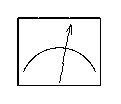
\includegraphics[scale=.5]{meter.eps}}~~~~}%
		\ar@{-}[l]}

%%%%%%%%%%%%%%%%%%%%%%%%%%%%%%%%%%%%%%%%%%%%%%%%%%%%%%%%%%%%%%%%%%%%%%%%%%%%%
% qubit names (and also revert to qubit wires, vs, cbit wires)

\def\q#1{*+{\rule[-0.2ex]{0ex}{2.1ex}|#1\>}}
\def\qv#1#2{*+{\rule[-0.2ex]{0ex}{2.1ex}|#1\>=|#2\>}}
	
%%%%%%%%%%%%%%%%%%%%%%%%%%%%%%%%%%%%%%%%%%%%%%%%%%%%%%%%%%%%%%%%%%%%%%%%%%%%%
% multiple qubit gates

% utulity text box for figuring out width of things
\newbox{\sbox}

% empty space of width determined by the text argument
\def\gspace#1{*+{\rule[-0.2ex]{0ex}{2.1ex}%
	\setbox\sbox=\hbox{$#1$}%
	\hspace*{\wd\sbox}}}
	
% n-qubit operation #1=box label, #2=number of qubits (eg d=2 qubits, ddd=4)
\def\gnqubit#1#2{\gspace{#1}
		 \save [].[#2]!C="qq"*[F]\frm{}\restore
		 \save "qq"*[]{#1} \restore}

% two-qubit operation
\def\gtwo#1{\gnqubit{#1}{d}}

% two-qubit operation
\def\gthree#1{\gnqubit{#1}{dd}}

%%%%%%%%%%%%%%%%%%%%%%%%%%%%%%%%%%%%%%%%%%%%%%%%%%%%%%%%%%%%%%%%%%%%%%%%%%%%%
% ``D'' style measurement gate a-la-cleve, at Michael Nielsen's request

\def\dmeterwide#1#2{*{\xy <0pt,-8pt>;<0pt,8pt> **@{-};
		    <0pt,-8pt>;<#2,-8pt> **@{-} ;
		    <0pt, 8pt>;<#2, 8pt> **@{-} ;
		    <#2,0pt>-<5pt,0pt>*{#1} ;
		    <#2,0pt>*\cir<8pt>{r_l}\endxy}}

\def\dmeter#1{\dmeterwide{#1}{12pt}}

%%%%%%%%%%%%%%%%%%%%%%%%%%%%%%%%%%%%%%%%%%%%%%%%%%%%%%%%%%%%%%%%%%%%%%%%%%%%%

% definitions for the circuit elements

\def\gAxA{\op{\txt{R\textsubscript{y}}}\w\A{gAxA}}
\def\gBxB{\gnqubit{\txt{H\textsubscript{ALL}}}{dd}\w\A{gBxB}}
\def\gBxC{\gspace{\txt{H\textsubscript{ALL}}}\w\A{gBxC}}
\def\gBxD{\gspace{\txt{H\textsubscript{ALL}}}\w\A{gBxD}}
\def\gBxA{\b\w\A{gBxA}}
\def\gCxA{\op{X}\w\A{gCxA}}
\def\gDxA{\b\w\A{gDxA}}
\def\gDxB{\op{\txt{R\textsubscript{y}}}\w\A{gDxB}}
\def\gExC{\gnqubit{\txt{H\textsubscript{ALL}}}{d}\w\A{gExC}}
\def\gExD{\gspace{\txt{H\textsubscript{ALL}}}\w\A{gExD}}
\def\gExA{\b\w\A{gExA}}
\def\gExB{\b\w\A{gExB}}
\def\gFxB{\op{X}\w\A{gFxB}}
\def\gGxA{\b\w\A{gGxA}}
\def\gGxB{\b\w\A{gGxB}}
\def\gGxC{\op{\txt{R\textsubscript{y}}}\w\A{gGxC}}
\def\gHxA{\b\w\A{gHxA}}
\def\gHxB{\b\w\A{gHxB}}
\def\gHxC{\b\w\A{gHxC}}
\def\gHxD{\op{\txt{H\textsubscript{ALL}}}\w\A{gHxD}}
\def\gIxC{\op{X}\w\A{gIxC}}
\def\gIxA{*-{}\w\A{gIxA}}
\def\gIxB{*-{}\w\A{gIxB}}
\def\gIxD{*-{}\w\A{gIxD}}
\def\gJxA{\meter\w\A{gJxA}}
\def\gJxB{\meter\w\A{gJxB}}
\def\gJxC{\meter\w\A{gJxC}}
\def\gJxD{\meter\w\A{gJxD}}

% definitions for bit labels and initial states

\def\bA{\qv{q_{0}}{0}}
\def\bB{\qv{q_{1}}{0}}
\def\bC{\qv{q_{2}}{0}}
\def\bD{\qv{q_{3}}{0}}

% The quantum circuit as an xymatrix


\xymatrix@R=5pt@C=10pt{
    \bA & \gAxA &\gBxA &\gCxA &\gDxA &\gExA &\n   &\gGxA &\gHxA &\gIxA &\gJxA &\N  
\\  \bB & \n   &\gBxB &\n   &\gDxB &\gExB &\gFxB &\gGxB &\gHxB &\gIxB &\gJxB &\N  
\\  \bC & \n   &\gBxC &\n   &\n   &\gExC &\n   &\gGxC &\gHxC &\gIxC &\gJxC &\N  
\\  \bD & \n   &\gBxD &\n   &\n   &\gExD &\n   &\n   &\gHxD &\gIxD &\gJxD &\N  
%
% Vertical lines and other post-xymatrix latex
%
\ar@{-}"gBxB";"gBxA"
\ar@{-}"gDxB";"gDxA"
\ar@{-}"gExC";"gExA"\ar@{-}"gExC";"gExB"
\ar@{-}"gGxC";"gGxA"\ar@{-}"gGxC";"gGxB"
\ar@{-}"gHxD";"gHxA"\ar@{-}"gHxD";"gHxB"\ar@{-}"gHxD";"gHxC"
}
% end qasm2circ

\end{document}